\documentclass[a4paper,10pt]{article}
\usepackage[utf8]{inputenc}
\usepackage{graphicx}
\usepackage{amsmath}
\usepackage{amssymb}
\usepackage{amsthm}
\usepackage{booktabs}
\usepackage{caption}
\usepackage{geometry}
%\usepackage{hyperref}
\usepackage{makeidx}
\usepackage{microtype}
\usepackage{subfig}
\usepackage{tabularx}
\usepackage{url}
\usepackage{varioref}
\usepackage[italian]{babel}
\usepackage{xcolor}
\usepackage{multicol}
\usepackage{mathtools}
\usepackage{booktabs}
\usepackage{gensymb}


\title{Laboratorio I: Misure di focali\\
\begin{large}
Dipartimento di Fisica E.Fermi - Università di Pisa
\end{large}}

\author{Di Ubaldo Gabriele \\Torosantucci Andrea}
\date{}

\begin{document}

\maketitle

\tableofcontents

%%%%%%%%%%%%%%%%%%%%%%%%%%%%%%%%%%%%%%%%%%%%%%%%%%%%%%%%%%%%%%%%%%%%%%%%%%%%%%%%%%%%%%%%%%%%%%%%%%%%%%%%%%%%%%%%%%%%%%%%%%%%%%%%%%%%%%%%%%%%%%%%%%%%%%%%%%%%%%%%%%%%%%%%%%%%%%%%%%%
\section{Introduzione}
\subsection{Teoria}
\textbf{Obiettivo:} Misurare le distanze focali di una lente convergente e una lente divergente.\\
Le lenti che studiamo sono descritte dall'ottica geometrica nell'approssimazione che esse siano sottili, cioè che il loro spessore sia molto minore del raggio luminoso.
In questo modello abbiamo che:
\begin{equation}
 \frac{1}{q}+\frac{1}{p}=\frac{1}{f}
\end{equation}
Per misurare la distanza focale di una lente divergente abbiamo bisogno di una lente convergente con potere diottrico maggiore in mudulo rispetto a quello della lenta divergente.
Useremo quindi una  sorgente virtuale per la lente divergente.
\subsection{Apparato sperimentale}
\begin{itemize}
\item{Banco ottico con sorgente luminosa}
\item{Schermo mobile e supporto per lenti}
\item{Set di lenti con varie lunghezze focali}
\item{Metro a nastro con risoluzione di $1mm$}
\end{itemize}

%%%%%%%%%%%%%%%%%%%%%%%%%%%%%%%%%%%%%%%%%%%%%%%%%%%%%%%%%%%%%%%%%%%%%%%%%%%%%%%%%%%%%%%%%%%%%%%%%%%%%%%%%%%%%%%%%%%%%%%%%%%%%%%%%%%%%%%%%%%%%%%%%%%%%%%%%%%%%%%%%%%%%%%%%%%%%%%%%%%
\section{Esperimento}
\subsection{Acquisizione misure}
\textbf{Convergente:} Fissiamo delle distanze arbitrarie $p_i$ e spostiamo lo schermo finchè non è a fuoco per misurare $q_i$. \\
\textbf{Divergente:} Posta la lente convergente sul banco ottico, mettiamo a fuoco sullo schermo e poi posizioniamo la lente divergente tra 
la convergente e lo schermo. Misuriamo la distanza $p_i$ con segno negativo  tra la divergente e lo schermo con l'immagine a fuoco della convergente  e poi rimettiamo a fuoco l'immagine secondo la divergente 
per misurare la distanza $q_i$.

All'inizio avevamo stimato il nostro errore sistematico come $0.5cm$ ma questo si è poi rivelato (dal test del $\chi2$), grazie alla precisione delle nostre misure,un errore troppo grande e abbiamo diminuito l'errore a $0.2$ per la convergente e $0.15$ per la divergente.

\subsection{Analisi Dati}
I dati misurati per la lente convergente  sono i seguenti:

\begin{table}[!htb]
\centering
\caption{Lente convergente}
\label{my-label}
\begin{tabular}{l|llllllllll}
$p(cm)$ & 25   & 28.1 & 33.1 & 43.7 & 47   & 51.1 & 37.2 & 27.2 & 40.4 & 49.4 \\ \cline{1-11} 
$q (cm)$     & 56.4 & 45.7 & 36.9 & 28.7 & 26.8 & 26.2 & 32.8 & 48.7 & 30.4 & 26.8 \\
\end{tabular}
\end{table}
 \begin {figure}[!htb]
\begin{center}
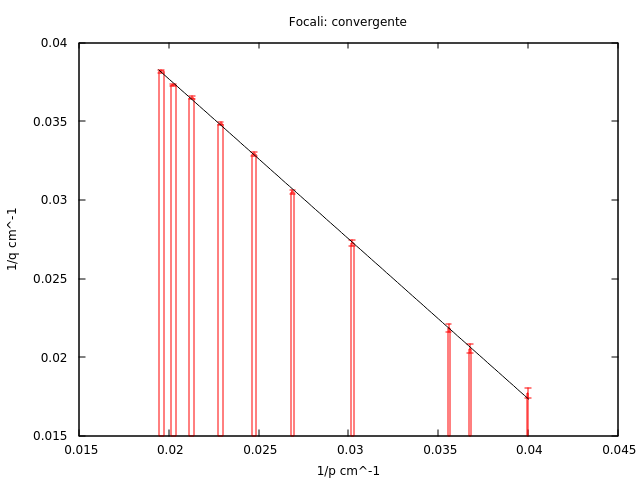
\includegraphics[width=10cm]{/home/zerch/Documents/UNIPI/LAB1/12Diottro/dati/graf-conv.png}
\end{center}
\end{figure}

I dati del fit della convergente sono i seguenti:
\begin{equation} 
\chi^2=8.53 \quad \chi^2_r=1.06 \quad a=-1.01\pm 0.009 \quad b=0.0580\pm0.0002
\end{equation}


I dati misurati per la lente divergente sono i seguenti:
\pagebreak
\begin{table}[!htb]
\centering
\caption{Lente divergente}
\label{my-label}
\begin{tabular}{l|lllllllll}
$p(cm)$ & 11.3  & 10.8 & 9.8 & 8.8 & 7.6 & 6.5 & 6.3 & 5.1 & 4.0  \\ \cline{1-10} 
$q (cm)$& 32.6 & 27.9 & 23.4 & 19.5 & 14.4 & 10.9 & 10.4 & 8.5 & 5.9 \\ 
\end{tabular}
\end{table}


 \begin {figure}[!htb]
\begin{center}
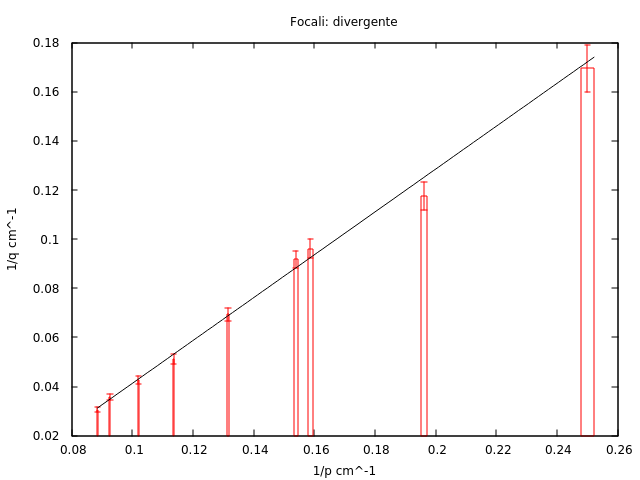
\includegraphics[width=10cm]{/home/zerch/Documents/UNIPI/LAB1/12Diottro/dati/graf-div.png}
\end{center}
\end{figure}


I dati del fit della divergente sono i seguenti:
\begin{equation} 
\chi^2= 5.56 \quad \chi^2_r=0.79 \quad a=0.87\pm 0.02 \quad	b=-0.046\pm0.003
\end{equation}

Il parametro $a$ dei fit deve essere vicino a 1 dato che rappresenta il coefficiente angolare della retta. Il parametro $b$ è l'inverso della lunghezza focale, cioè il potere diottrico. Nella lente convergente $a$ è compatibile con $1$ mentre per la divergente no. Questo è dovuto probabilmente al ristretto numero di misure e agli errori alti per $p$ bassi.

(se ti va fai la somma del chi2 aggiungendo l'errore sulla x a mano)
\section{Conclusione}
Il test del $\chi^2$ conferma la validità del nostro modello fisico in entrambi i casi.
Nella convergente la lunghezza focale è $f=172.2\pm0.6mm$ che dimostra con certezza che la lunghezza focale dichiarata dal rivenditore di $150mm$ non  è corretta.
Nella divergente la lunghezza focale è $f=217.4\pm1.2mm$ che dimostra anche per la divergente che la lunghezza focale dichiarata dal rivenditore di $200$ non è corretta.
L'esperimento ha avuto successo sia nel misurare le caratteristiche delle lenti sia nel testare il nostro modello.
\end{document}



8
7
6
5
4